\begin{enumerate}[label=\thesection.\arabic*.,ref=\thesection.\theenumi]
\numberwithin{equation}{enumi}
\item
\textbf{Question}
In the feedback system given below 
\begin{align}
G(s) = \frac{1}{(s+1)(s+2)(s+3)}
\end{align}

The positive value of k for which the gain margin of system is exactly 0 dB and phase margin of system is exactly 0 degree is?
\begin{figure}[!ht]
	\begin{center}
		
		\resizebox{\columnwidth}{!}{\begin{enumerate}[label=\thesection.\arabic*.,ref=\thesection.\theenumi]
\numberwithin{equation}{enumi}

\item
\textbf{Question}
In the feedback system given below 
\begin{align}
G(s) = \frac{1}{(s+1)(s+2)(s+3)}
\end{align}

The positive value of k for which the gain margin of system is exactly 0 dB and phase margin of system is exactly 0 degree is?
\begin{figure}[!ht]
	\begin{center}
		
		\resizebox{\columnwidth}{!}{\begin{enumerate}[label=\thesection.\arabic*.,ref=\thesection.\theenumi]
\numberwithin{equation}{enumi}

\item
\textbf{Question}
In the feedback system given below 
\begin{align}
G(s) = \frac{1}{(s+1)(s+2)(s+3)}
\end{align}

The positive value of k for which the gain margin of system is exactly 0 dB and phase margin of system is exactly 0 degree is?
\begin{figure}[!ht]
	\begin{center}
		
		\resizebox{\columnwidth}{!}{\begin{enumerate}[label=\thesection.\arabic*.,ref=\thesection.\theenumi]
\numberwithin{equation}{enumi}

\item
\textbf{Question}
In the feedback system given below 
\begin{align}
G(s) = \frac{1}{(s+1)(s+2)(s+3)}
\end{align}

The positive value of k for which the gain margin of system is exactly 0 dB and phase margin of system is exactly 0 degree is?
\begin{figure}[!ht]
	\begin{center}
		
		\resizebox{\columnwidth}{!}{\input{./figs/ee18btech11036.tex}}
	\end{center}
\caption{}
\label{fig:ee18btech11036}
\end{figure}

\ref{fig:ee18btech11036}


\item
% \begin{frame}{Question}
% \begin{block}


% \end{block}
% \end{frame}
% % \begin{frame}
% % \tableofcontents
% % \end{frame}

% \begin{frame}{Theory}

% \begin{block}

% \end{block} \vspace{16pt}




% \end{frame}


\input{figs/ee18btech11036.tikz}
\item
\textbf{Technique description}
As given in question we see that gain margin is 0 dB and phase margin is 0 degrees. This implies that system is just enough stable and will become destabilized on just small increase in gain. Hence the system is marginbally stable.
% \end{block}
% \end{frame}
% \begin{frame}
% \begin{block}


The stability of the system can be checked by Routh-Hurwitz Stability Criterion 
% \end{block}

% \end{frame}

\item
% \begin{frame}{Routh-Hurwitz Stability Criterion}
% \begin{block}
\textbf{Routh Hurwitz Criterion}
Sufficient condition for Routh-Hurwitz Stability Criterion:The sufficient condition is that all the elements of the first column of the Routh array should have the same sign. This means that all the elements of the first column of the Routh array should be either positive or negative.\vspace{16pt}
% \includegraphics[scale=0.3]{pic2}
% \end{block}

% \end{frame}

%\begin{frame}
\begin{figure}
\centering
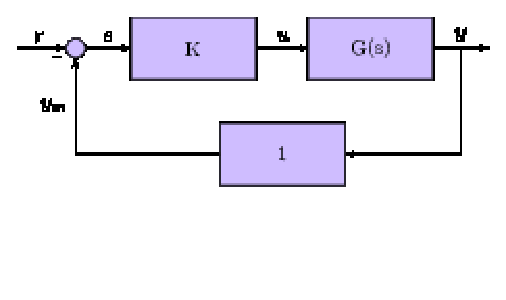
\includegraphics[width=\columnwidth]{./figs/ee18btech11036.tex}
\end{figure}



\item
the Routh array for characteristic equation
\begin{multline}
q(s) = a_0s^n+a_1s^{n-1}+.....+a_{n-1}s+a_n = 0
\end{multline}
 can be constructed as:
 
\begin{align}
\mydet{s^n\\s^{n-1}\\s^{n-2} \\ \vdots}
 \mydet{a_0 & a_2 & a_4 & \cdots \\
a_1 & a_3 & a_5 & \cdots  \\
b_1 & b_2 & b_3 & \cdots \\
\vdots & \vdots & \vdots & \ddots &\vdots 
 \cdots \\}
\end{align}
%
 where
 \begin{align}
 b_1 =\frac{ a_1a_2-a_0a_3}{a_1}  
 \\
 b_2 =\frac{ a_1a_4-a_0a_5}{a_1} 
 \\
 c_1=\frac{ b_1a_3-a_1b_2}{b_1} 
\\
 c_2=\frac{ b_1a_5-a_1b_3}{b_1}  
\end{align}



% \begin{frame}{Solution}
\item
\textbf{Solution}
The Routh array for equation 
\begin{align}
s^3+6s^2+11s^1+(6+k)
\end{align}

\begin{align}
\mydet{s^3\\s^2\\s^1 \\ s^0}
\mydet{1 & 11 \\ 6 & (6+k) \\  \frac{66-(6+k)}{6} & 0\\ (6+k) & 0}
\end{align}

\item
Now since the system is marginally stable therefore $s^1$ row is $\geq$ 0\newline
So 
\begin{align}
    \frac{66-(6+K)}{6}>0
\end{align}

Hence
\begin{align}
k=60
\end{align}
%\end{frame}
\item
\includegraphics[scale=0.18]{./plots/nyq.png}


\begin{frame}{Verification using Plots}
\includegraphics[scale=0.18]{./plots/nyq_zoomed.png}

\end{frame}

\end{enumerate}





}
	\end{center}
\caption{}
\label{fig:ee18btech11036}
\end{figure}

\ref{fig:ee18btech11036}


\item
% \begin{frame}{Question}
% \begin{block}


% \end{block}
% \end{frame}
% % \begin{frame}
% % \tableofcontents
% % \end{frame}

% \begin{frame}{Theory}

% \begin{block}

% \end{block} \vspace{16pt}




% \end{frame}


\begin{enumerate}[label=\thesection.\arabic*.,ref=\thesection.\theenumi]
\numberwithin{equation}{enumi}

\item
\textbf{Question}
In the feedback system given below 
\begin{align}
G(s) = \frac{1}{(s+1)(s+2)(s+3)}
\end{align}

The positive value of k for which the gain margin of system is exactly 0 dB and phase margin of system is exactly 0 degree is?
\begin{figure}[!ht]
	\begin{center}
		
		\resizebox{\columnwidth}{!}{\input{./figs/ee18btech11036.tex}}
	\end{center}
\caption{}
\label{fig:ee18btech11036}
\end{figure}

\ref{fig:ee18btech11036}


\item
% \begin{frame}{Question}
% \begin{block}


% \end{block}
% \end{frame}
% % \begin{frame}
% % \tableofcontents
% % \end{frame}

% \begin{frame}{Theory}

% \begin{block}

% \end{block} \vspace{16pt}




% \end{frame}


\input{figs/ee18btech11036.tikz}
\item
\textbf{Technique description}
As given in question we see that gain margin is 0 dB and phase margin is 0 degrees. This implies that system is just enough stable and will become destabilized on just small increase in gain. Hence the system is marginbally stable.
% \end{block}
% \end{frame}
% \begin{frame}
% \begin{block}


The stability of the system can be checked by Routh-Hurwitz Stability Criterion 
% \end{block}

% \end{frame}

\item
% \begin{frame}{Routh-Hurwitz Stability Criterion}
% \begin{block}
\textbf{Routh Hurwitz Criterion}
Sufficient condition for Routh-Hurwitz Stability Criterion:The sufficient condition is that all the elements of the first column of the Routh array should have the same sign. This means that all the elements of the first column of the Routh array should be either positive or negative.\vspace{16pt}
% \includegraphics[scale=0.3]{pic2}
% \end{block}

% \end{frame}

%\begin{frame}
\begin{figure}
\centering
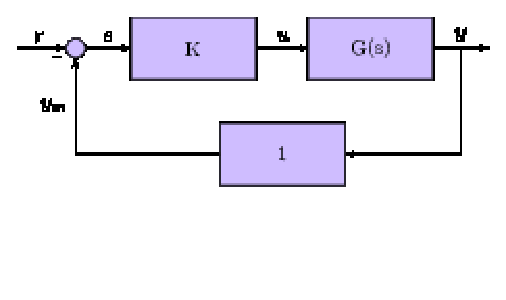
\includegraphics[width=\columnwidth]{./figs/ee18btech11036.tex}
\end{figure}



\item
the Routh array for characteristic equation
\begin{multline}
q(s) = a_0s^n+a_1s^{n-1}+.....+a_{n-1}s+a_n = 0
\end{multline}
 can be constructed as:
 
\begin{align}
\mydet{s^n\\s^{n-1}\\s^{n-2} \\ \vdots}
 \mydet{a_0 & a_2 & a_4 & \cdots \\
a_1 & a_3 & a_5 & \cdots  \\
b_1 & b_2 & b_3 & \cdots \\
\vdots & \vdots & \vdots & \ddots &\vdots 
 \cdots \\}
\end{align}
%
 where
 \begin{align}
 b_1 =\frac{ a_1a_2-a_0a_3}{a_1}  
 \\
 b_2 =\frac{ a_1a_4-a_0a_5}{a_1} 
 \\
 c_1=\frac{ b_1a_3-a_1b_2}{b_1} 
\\
 c_2=\frac{ b_1a_5-a_1b_3}{b_1}  
\end{align}



% \begin{frame}{Solution}
\item
\textbf{Solution}
The Routh array for equation 
\begin{align}
s^3+6s^2+11s^1+(6+k)
\end{align}

\begin{align}
\mydet{s^3\\s^2\\s^1 \\ s^0}
\mydet{1 & 11 \\ 6 & (6+k) \\  \frac{66-(6+k)}{6} & 0\\ (6+k) & 0}
\end{align}

\item
Now since the system is marginally stable therefore $s^1$ row is $\geq$ 0\newline
So 
\begin{align}
    \frac{66-(6+K)}{6}>0
\end{align}

Hence
\begin{align}
k=60
\end{align}
%\end{frame}
\item
\includegraphics[scale=0.18]{./plots/nyq.png}


\begin{frame}{Verification using Plots}
\includegraphics[scale=0.18]{./plots/nyq_zoomed.png}

\end{frame}

\end{enumerate}






\item
\textbf{Technique description}
As given in question we see that gain margin is 0 dB and phase margin is 0 degrees. This implies that system is just enough stable and will become destabilized on just small increase in gain. Hence the system is marginbally stable.
% \end{block}
% \end{frame}
% \begin{frame}
% \begin{block}


The stability of the system can be checked by Routh-Hurwitz Stability Criterion 
% \end{block}

% \end{frame}

\item
% \begin{frame}{Routh-Hurwitz Stability Criterion}
% \begin{block}
\textbf{Routh Hurwitz Criterion}
Sufficient condition for Routh-Hurwitz Stability Criterion:The sufficient condition is that all the elements of the first column of the Routh array should have the same sign. This means that all the elements of the first column of the Routh array should be either positive or negative.\vspace{16pt}
% \includegraphics[scale=0.3]{pic2}
% \end{block}

% \end{frame}

%\begin{frame}
\begin{figure}
\centering
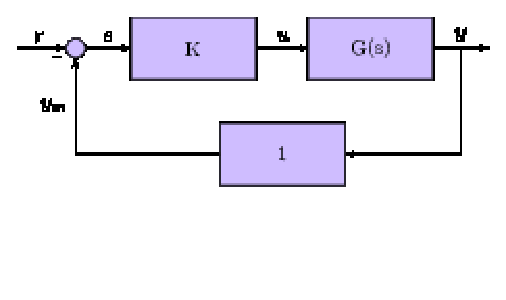
\includegraphics[width=\columnwidth]{./figs/ee18btech11036.tex}
\end{figure}



\item
the Routh array for characteristic equation
\begin{multline}
q(s) = a_0s^n+a_1s^{n-1}+.....+a_{n-1}s+a_n = 0
\end{multline}
 can be constructed as:
 
\begin{align}
\mydet{s^n\\s^{n-1}\\s^{n-2} \\ \vdots}
 \mydet{a_0 & a_2 & a_4 & \cdots \\
a_1 & a_3 & a_5 & \cdots  \\
b_1 & b_2 & b_3 & \cdots \\
\vdots & \vdots & \vdots & \ddots &\vdots 
 \cdots \\}
\end{align}
%
 where
 \begin{align}
 b_1 =\frac{ a_1a_2-a_0a_3}{a_1}  
 \\
 b_2 =\frac{ a_1a_4-a_0a_5}{a_1} 
 \\
 c_1=\frac{ b_1a_3-a_1b_2}{b_1} 
\\
 c_2=\frac{ b_1a_5-a_1b_3}{b_1}  
\end{align}



% \begin{frame}{Solution}
\item
\textbf{Solution}
The Routh array for equation 
\begin{align}
s^3+6s^2+11s^1+(6+k)
\end{align}

\begin{align}
\mydet{s^3\\s^2\\s^1 \\ s^0}
\mydet{1 & 11 \\ 6 & (6+k) \\  \frac{66-(6+k)}{6} & 0\\ (6+k) & 0}
\end{align}

\item
Now since the system is marginally stable therefore $s^1$ row is $\geq$ 0\newline
So 
\begin{align}
    \frac{66-(6+K)}{6}>0
\end{align}

Hence
\begin{align}
k=60
\end{align}
%\end{frame}
\item
\includegraphics[scale=0.18]{./plots/nyq.png}


\begin{frame}{Verification using Plots}
\includegraphics[scale=0.18]{./plots/nyq_zoomed.png}

\end{frame}

\end{enumerate}





}
	\end{center}
\caption{}
\label{fig:ee18btech11036}
\end{figure}

\ref{fig:ee18btech11036}


\item
% \begin{frame}{Question}
% \begin{block}


% \end{block}
% \end{frame}
% % \begin{frame}
% % \tableofcontents
% % \end{frame}

% \begin{frame}{Theory}

% \begin{block}

% \end{block} \vspace{16pt}




% \end{frame}


\begin{enumerate}[label=\thesection.\arabic*.,ref=\thesection.\theenumi]
\numberwithin{equation}{enumi}

\item
\textbf{Question}
In the feedback system given below 
\begin{align}
G(s) = \frac{1}{(s+1)(s+2)(s+3)}
\end{align}

The positive value of k for which the gain margin of system is exactly 0 dB and phase margin of system is exactly 0 degree is?
\begin{figure}[!ht]
	\begin{center}
		
		\resizebox{\columnwidth}{!}{\begin{enumerate}[label=\thesection.\arabic*.,ref=\thesection.\theenumi]
\numberwithin{equation}{enumi}

\item
\textbf{Question}
In the feedback system given below 
\begin{align}
G(s) = \frac{1}{(s+1)(s+2)(s+3)}
\end{align}

The positive value of k for which the gain margin of system is exactly 0 dB and phase margin of system is exactly 0 degree is?
\begin{figure}[!ht]
	\begin{center}
		
		\resizebox{\columnwidth}{!}{\input{./figs/ee18btech11036.tex}}
	\end{center}
\caption{}
\label{fig:ee18btech11036}
\end{figure}

\ref{fig:ee18btech11036}


\item
% \begin{frame}{Question}
% \begin{block}


% \end{block}
% \end{frame}
% % \begin{frame}
% % \tableofcontents
% % \end{frame}

% \begin{frame}{Theory}

% \begin{block}

% \end{block} \vspace{16pt}




% \end{frame}


\input{figs/ee18btech11036.tikz}
\item
\textbf{Technique description}
As given in question we see that gain margin is 0 dB and phase margin is 0 degrees. This implies that system is just enough stable and will become destabilized on just small increase in gain. Hence the system is marginbally stable.
% \end{block}
% \end{frame}
% \begin{frame}
% \begin{block}


The stability of the system can be checked by Routh-Hurwitz Stability Criterion 
% \end{block}

% \end{frame}

\item
% \begin{frame}{Routh-Hurwitz Stability Criterion}
% \begin{block}
\textbf{Routh Hurwitz Criterion}
Sufficient condition for Routh-Hurwitz Stability Criterion:The sufficient condition is that all the elements of the first column of the Routh array should have the same sign. This means that all the elements of the first column of the Routh array should be either positive or negative.\vspace{16pt}
% \includegraphics[scale=0.3]{pic2}
% \end{block}

% \end{frame}

%\begin{frame}
\begin{figure}
\centering
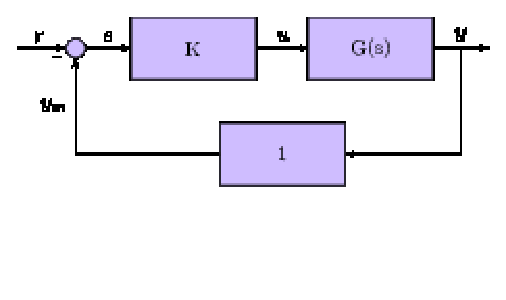
\includegraphics[width=\columnwidth]{./figs/ee18btech11036.tex}
\end{figure}



\item
the Routh array for characteristic equation
\begin{multline}
q(s) = a_0s^n+a_1s^{n-1}+.....+a_{n-1}s+a_n = 0
\end{multline}
 can be constructed as:
 
\begin{align}
\mydet{s^n\\s^{n-1}\\s^{n-2} \\ \vdots}
 \mydet{a_0 & a_2 & a_4 & \cdots \\
a_1 & a_3 & a_5 & \cdots  \\
b_1 & b_2 & b_3 & \cdots \\
\vdots & \vdots & \vdots & \ddots &\vdots 
 \cdots \\}
\end{align}
%
 where
 \begin{align}
 b_1 =\frac{ a_1a_2-a_0a_3}{a_1}  
 \\
 b_2 =\frac{ a_1a_4-a_0a_5}{a_1} 
 \\
 c_1=\frac{ b_1a_3-a_1b_2}{b_1} 
\\
 c_2=\frac{ b_1a_5-a_1b_3}{b_1}  
\end{align}



% \begin{frame}{Solution}
\item
\textbf{Solution}
The Routh array for equation 
\begin{align}
s^3+6s^2+11s^1+(6+k)
\end{align}

\begin{align}
\mydet{s^3\\s^2\\s^1 \\ s^0}
\mydet{1 & 11 \\ 6 & (6+k) \\  \frac{66-(6+k)}{6} & 0\\ (6+k) & 0}
\end{align}

\item
Now since the system is marginally stable therefore $s^1$ row is $\geq$ 0\newline
So 
\begin{align}
    \frac{66-(6+K)}{6}>0
\end{align}

Hence
\begin{align}
k=60
\end{align}
%\end{frame}
\item
\includegraphics[scale=0.18]{./plots/nyq.png}


\begin{frame}{Verification using Plots}
\includegraphics[scale=0.18]{./plots/nyq_zoomed.png}

\end{frame}

\end{enumerate}





}
	\end{center}
\caption{}
\label{fig:ee18btech11036}
\end{figure}

\ref{fig:ee18btech11036}


\item
% \begin{frame}{Question}
% \begin{block}


% \end{block}
% \end{frame}
% % \begin{frame}
% % \tableofcontents
% % \end{frame}

% \begin{frame}{Theory}

% \begin{block}

% \end{block} \vspace{16pt}




% \end{frame}


\begin{enumerate}[label=\thesection.\arabic*.,ref=\thesection.\theenumi]
\numberwithin{equation}{enumi}

\item
\textbf{Question}
In the feedback system given below 
\begin{align}
G(s) = \frac{1}{(s+1)(s+2)(s+3)}
\end{align}

The positive value of k for which the gain margin of system is exactly 0 dB and phase margin of system is exactly 0 degree is?
\begin{figure}[!ht]
	\begin{center}
		
		\resizebox{\columnwidth}{!}{\input{./figs/ee18btech11036.tex}}
	\end{center}
\caption{}
\label{fig:ee18btech11036}
\end{figure}

\ref{fig:ee18btech11036}


\item
% \begin{frame}{Question}
% \begin{block}


% \end{block}
% \end{frame}
% % \begin{frame}
% % \tableofcontents
% % \end{frame}

% \begin{frame}{Theory}

% \begin{block}

% \end{block} \vspace{16pt}




% \end{frame}


\input{figs/ee18btech11036.tikz}
\item
\textbf{Technique description}
As given in question we see that gain margin is 0 dB and phase margin is 0 degrees. This implies that system is just enough stable and will become destabilized on just small increase in gain. Hence the system is marginbally stable.
% \end{block}
% \end{frame}
% \begin{frame}
% \begin{block}


The stability of the system can be checked by Routh-Hurwitz Stability Criterion 
% \end{block}

% \end{frame}

\item
% \begin{frame}{Routh-Hurwitz Stability Criterion}
% \begin{block}
\textbf{Routh Hurwitz Criterion}
Sufficient condition for Routh-Hurwitz Stability Criterion:The sufficient condition is that all the elements of the first column of the Routh array should have the same sign. This means that all the elements of the first column of the Routh array should be either positive or negative.\vspace{16pt}
% \includegraphics[scale=0.3]{pic2}
% \end{block}

% \end{frame}

%\begin{frame}
\begin{figure}
\centering
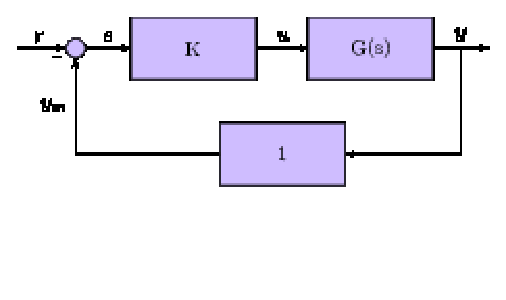
\includegraphics[width=\columnwidth]{./figs/ee18btech11036.tex}
\end{figure}



\item
the Routh array for characteristic equation
\begin{multline}
q(s) = a_0s^n+a_1s^{n-1}+.....+a_{n-1}s+a_n = 0
\end{multline}
 can be constructed as:
 
\begin{align}
\mydet{s^n\\s^{n-1}\\s^{n-2} \\ \vdots}
 \mydet{a_0 & a_2 & a_4 & \cdots \\
a_1 & a_3 & a_5 & \cdots  \\
b_1 & b_2 & b_3 & \cdots \\
\vdots & \vdots & \vdots & \ddots &\vdots 
 \cdots \\}
\end{align}
%
 where
 \begin{align}
 b_1 =\frac{ a_1a_2-a_0a_3}{a_1}  
 \\
 b_2 =\frac{ a_1a_4-a_0a_5}{a_1} 
 \\
 c_1=\frac{ b_1a_3-a_1b_2}{b_1} 
\\
 c_2=\frac{ b_1a_5-a_1b_3}{b_1}  
\end{align}



% \begin{frame}{Solution}
\item
\textbf{Solution}
The Routh array for equation 
\begin{align}
s^3+6s^2+11s^1+(6+k)
\end{align}

\begin{align}
\mydet{s^3\\s^2\\s^1 \\ s^0}
\mydet{1 & 11 \\ 6 & (6+k) \\  \frac{66-(6+k)}{6} & 0\\ (6+k) & 0}
\end{align}

\item
Now since the system is marginally stable therefore $s^1$ row is $\geq$ 0\newline
So 
\begin{align}
    \frac{66-(6+K)}{6}>0
\end{align}

Hence
\begin{align}
k=60
\end{align}
%\end{frame}
\item
\includegraphics[scale=0.18]{./plots/nyq.png}


\begin{frame}{Verification using Plots}
\includegraphics[scale=0.18]{./plots/nyq_zoomed.png}

\end{frame}

\end{enumerate}






\item
\textbf{Technique description}
As given in question we see that gain margin is 0 dB and phase margin is 0 degrees. This implies that system is just enough stable and will become destabilized on just small increase in gain. Hence the system is marginbally stable.
% \end{block}
% \end{frame}
% \begin{frame}
% \begin{block}


The stability of the system can be checked by Routh-Hurwitz Stability Criterion 
% \end{block}

% \end{frame}

\item
% \begin{frame}{Routh-Hurwitz Stability Criterion}
% \begin{block}
\textbf{Routh Hurwitz Criterion}
Sufficient condition for Routh-Hurwitz Stability Criterion:The sufficient condition is that all the elements of the first column of the Routh array should have the same sign. This means that all the elements of the first column of the Routh array should be either positive or negative.\vspace{16pt}
% \includegraphics[scale=0.3]{pic2}
% \end{block}

% \end{frame}

%\begin{frame}
\begin{figure}
\centering
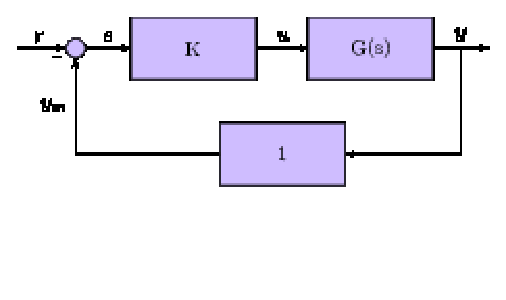
\includegraphics[width=\columnwidth]{./figs/ee18btech11036.tex}
\end{figure}



\item
the Routh array for characteristic equation
\begin{multline}
q(s) = a_0s^n+a_1s^{n-1}+.....+a_{n-1}s+a_n = 0
\end{multline}
 can be constructed as:
 
\begin{align}
\mydet{s^n\\s^{n-1}\\s^{n-2} \\ \vdots}
 \mydet{a_0 & a_2 & a_4 & \cdots \\
a_1 & a_3 & a_5 & \cdots  \\
b_1 & b_2 & b_3 & \cdots \\
\vdots & \vdots & \vdots & \ddots &\vdots 
 \cdots \\}
\end{align}
%
 where
 \begin{align}
 b_1 =\frac{ a_1a_2-a_0a_3}{a_1}  
 \\
 b_2 =\frac{ a_1a_4-a_0a_5}{a_1} 
 \\
 c_1=\frac{ b_1a_3-a_1b_2}{b_1} 
\\
 c_2=\frac{ b_1a_5-a_1b_3}{b_1}  
\end{align}



% \begin{frame}{Solution}
\item
\textbf{Solution}
The Routh array for equation 
\begin{align}
s^3+6s^2+11s^1+(6+k)
\end{align}

\begin{align}
\mydet{s^3\\s^2\\s^1 \\ s^0}
\mydet{1 & 11 \\ 6 & (6+k) \\  \frac{66-(6+k)}{6} & 0\\ (6+k) & 0}
\end{align}

\item
Now since the system is marginally stable therefore $s^1$ row is $\geq$ 0\newline
So 
\begin{align}
    \frac{66-(6+K)}{6}>0
\end{align}

Hence
\begin{align}
k=60
\end{align}
%\end{frame}
\item
\includegraphics[scale=0.18]{./plots/nyq.png}


\begin{frame}{Verification using Plots}
\includegraphics[scale=0.18]{./plots/nyq_zoomed.png}

\end{frame}

\end{enumerate}






\item
\textbf{Technique description}
As given in question we see that gain margin is 0 dB and phase margin is 0 degrees. This implies that system is just enough stable and will become destabilized on just small increase in gain. Hence the system is marginbally stable.
% \end{block}
% \end{frame}
% \begin{frame}
% \begin{block}


The stability of the system can be checked by Routh-Hurwitz Stability Criterion 
% \end{block}

% \end{frame}

\item
% \begin{frame}{Routh-Hurwitz Stability Criterion}
% \begin{block}
\textbf{Routh Hurwitz Criterion}
Sufficient condition for Routh-Hurwitz Stability Criterion:The sufficient condition is that all the elements of the first column of the Routh array should have the same sign. This means that all the elements of the first column of the Routh array should be either positive or negative.\vspace{16pt}
% \includegraphics[scale=0.3]{pic2}
% \end{block}

% \end{frame}

%\begin{frame}
\begin{figure}
\centering
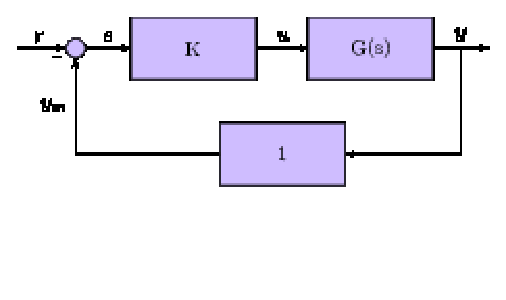
\includegraphics[width=\columnwidth]{./figs/ee18btech11036.tex}
\end{figure}



\item
the Routh array for characteristic equation
\begin{multline}
q(s) = a_0s^n+a_1s^{n-1}+.....+a_{n-1}s+a_n = 0
\end{multline}
 can be constructed as:
 
\begin{align}
\mydet{s^n\\s^{n-1}\\s^{n-2} \\ \vdots}
 \mydet{a_0 & a_2 & a_4 & \cdots \\
a_1 & a_3 & a_5 & \cdots  \\
b_1 & b_2 & b_3 & \cdots \\
\vdots & \vdots & \vdots & \ddots &\vdots 
 \cdots \\}
\end{align}
%
 where
 \begin{align}
 b_1 =\frac{ a_1a_2-a_0a_3}{a_1}  
 \\
 b_2 =\frac{ a_1a_4-a_0a_5}{a_1} 
 \\
 c_1=\frac{ b_1a_3-a_1b_2}{b_1} 
\\
 c_2=\frac{ b_1a_5-a_1b_3}{b_1}  
\end{align}



% \begin{frame}{Solution}
\item
\textbf{Solution}
The Routh array for equation 
\begin{align}
s^3+6s^2+11s^1+(6+k)
\end{align}

\begin{align}
\mydet{s^3\\s^2\\s^1 \\ s^0}
\mydet{1 & 11 \\ 6 & (6+k) \\  \frac{66-(6+k)}{6} & 0\\ (6+k) & 0}
\end{align}

\item
Now since the system is marginally stable therefore $s^1$ row is $\geq$ 0\newline
So 
\begin{align}
    \frac{66-(6+K)}{6}>0
\end{align}

Hence
\begin{align}
k=60
\end{align}
%\end{frame}
\item
\includegraphics[scale=0.18]{./plots/nyq.png}


\begin{frame}{Verification using Plots}
\includegraphics[scale=0.18]{./plots/nyq_zoomed.png}

\end{frame}

\end{enumerate}





}
	\end{center}
\caption{}
\label{fig:ee18btech11036}
\end{figure}

\ref{fig:ee18btech11036}

\begin{figure}
\centering
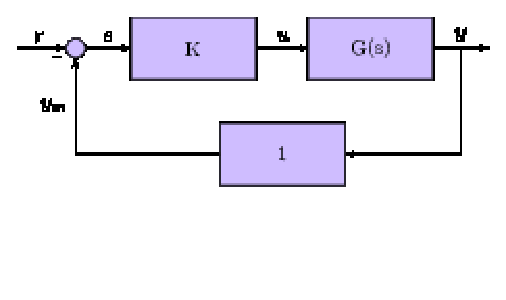
\includegraphics[width=\columnwidth]{./figs/ee18btech11036.eps}
\end{figure}
\item
% \begin{frame}{Question}
% \begin{block}


% \end{block}
% \end{frame}
% % \begin{frame}
% % \tableofcontents
% % \end{frame}

% \begin{frame}{Theory}

% \begin{block}
\textbf{Theory}
\newline
\textbf{Gain Margin}
The gain margin is defined as the change in open-loop gain required to make the closed-loop system unstable. Systems with greater gain margins can withstand greater changes in system parameters before becoming unstable in closed-loop. 

% \end{block} \vspace{16pt}
% \begin{block}
\textbf{Phase Margin}
The phase margin is defined as the change in open-loop phase shift required to make the closed-loop system unstable. The phase margin also measures the system's tolerance to time delay
% \end{block} \vspace{16pt}




% \end{frame}



\item
\textbf{Technique description}
As given in question we see that gain margin is 0 dB and phase margin is 0 degrees. This implies that system is just enough stable and will become destabilized on just small increase in gain. Hence the system is marginbally stable.
% \end{block}
% \end{frame}
% \begin{frame}
% \begin{block}


The stability of the system can be checked by Routh-Hurwitz Stability Criterion 
% \end{block}

% \end{frame}

\item
% \begin{frame}{Routh-Hurwitz Stability Criterion}
% \begin{block}
\textbf{Routh Hurwitz Criterion}
Necessary condition for Routh-Hurwitz Stability Criterion: The necessary condition is that the coefficients of the characteristic polynomial should be positive. This implies that all the roots of the characteristic equation should have negative real parts.

Sufficient condition for Routh-Hurwitz Stability Criterion:The sufficient condition is that all the elements of the first column of the Routh array should have the same sign. This means that all the elements of the first column of the Routh array should be either positive or negative.\vspace{16pt}
% \includegraphics[scale=0.3]{pic2}
% \end{block}

% \end{frame}

%\begin{frame}
\item
The Routh array for characteristic equation $a_0$s^n+$a_1$s^{n-1}+$a_2$s^{n-2}+.....+$a_{n-1}$s+$a_n$ = 0
\newline
\begin{vmatrix}s^n\\s^{n-1}\\s^{n-2} \\ \vdots \end{vmatrix} \begin{vmatrix}
a_0 & a_2 & a_4 & \cdots \\
a_1 & a_3 & a_5 & \cdots  \\
b_1 & b_2 & b_3 & \cdots \\
\vdots & \vdots & \vdots & \ddots &\vdots 
 \cdots \\ \end{vmatrix} 
 \newline
 where b_1 =\frac{ a_1a_2-a_0a_3}{a_1}  \hspace{5pt} b_2 =\frac{ a_1a_4-a_0a_5}{a_1} \hspace{5pt} c_1=\frac{ b_1a_3-a_1b_2}{b_1}  \hspace{5pt}     c_2=\frac{ b_1a_5-a_1b_3}{b_1} 
%\end{frame}

% \begin{frame}{Solution}
\item
\textbf{Solution}
The Routh array for equation $s^3+6s^2+11s^1+(6+k)$

\begin{tabular}{lllll}
$s^3$ & 1            & 11    &  &  \\
$s^2$ & 6            & (6+k) &  &  \\
$s^1$ & $\frac{66-(6+K)}{6}$& 0     &  &  \\
$s^0$ & $(6+k)$        & 0     &  & 


\end{tabular}

\item
Now since the system is marginally stable therefore $s^1$ row is $\geq$ 0\newline
Hence $\frac{66-(6+K)}{6}$
Hence k=60
%\end{frame}
\item
\includegraphics[scale=0.18]{./plots/nyq.png}


\begin{frame}{Verification using Plots}
\includegraphics[scale=0.18]{./plots/nyq_zoomed.png}

\end{frame}

\end{enumerate}





